\documentclass{article}
\usepackage[utf8]{inputenc}
\usepackage{amsmath,amssymb,graphicx}
\usepackage{cleveref}

\usepackage{listings}
\usepackage{color}

\lstnewenvironment{python}[1][]{
  \lstset{
    language=python,
    breaklines=true,
    tabsize=4,
    basicstyle=\ttfamily\small,
    otherkeywords={1, 2, 3, 4, 5, 6, 7, 8 ,9 , 0, -, =, +, [, ], (, ), \{, \}, :, *, !},
    keywordstyle=\color{blue},
    stringstyle=\color{red},
    showstringspaces=false,
    emph={class, pass, in, for, while, if, is, elif, else, not, and, or, OR
    def, print, exec, break, continue, return},
    emphstyle=\color{black}\bfseries,
    emph={[2]True, False, None, self},
    emphstyle=[2]\color{key},
    emph={[3]from, import, as},
    emphstyle=[3]\color{blue},
    morecomment=[s]{"""}{"""},
    commentstyle=\color{gray}\slshape,
    rulesepcolor=\color{blue},#1
  }
}{}

\title{Insert Assignment Title Here\\02807 Computational Tools for Big Data}
\author{Anonymous authors}
\date{Insert hand in date here}

\begin{document}

\maketitle

\section{Exercise 1.1}
You can put text in here. And formulas $e=mc^2$ and even big formulas:
\[
\sum_{n=2}^{\infty} \frac{1}{n^2} = 1
\]

\section{Exercise 1.2}
And you can put images in here and reference them like \Cref{fig:my_label}.

\begin{figure}[!h]
\centering
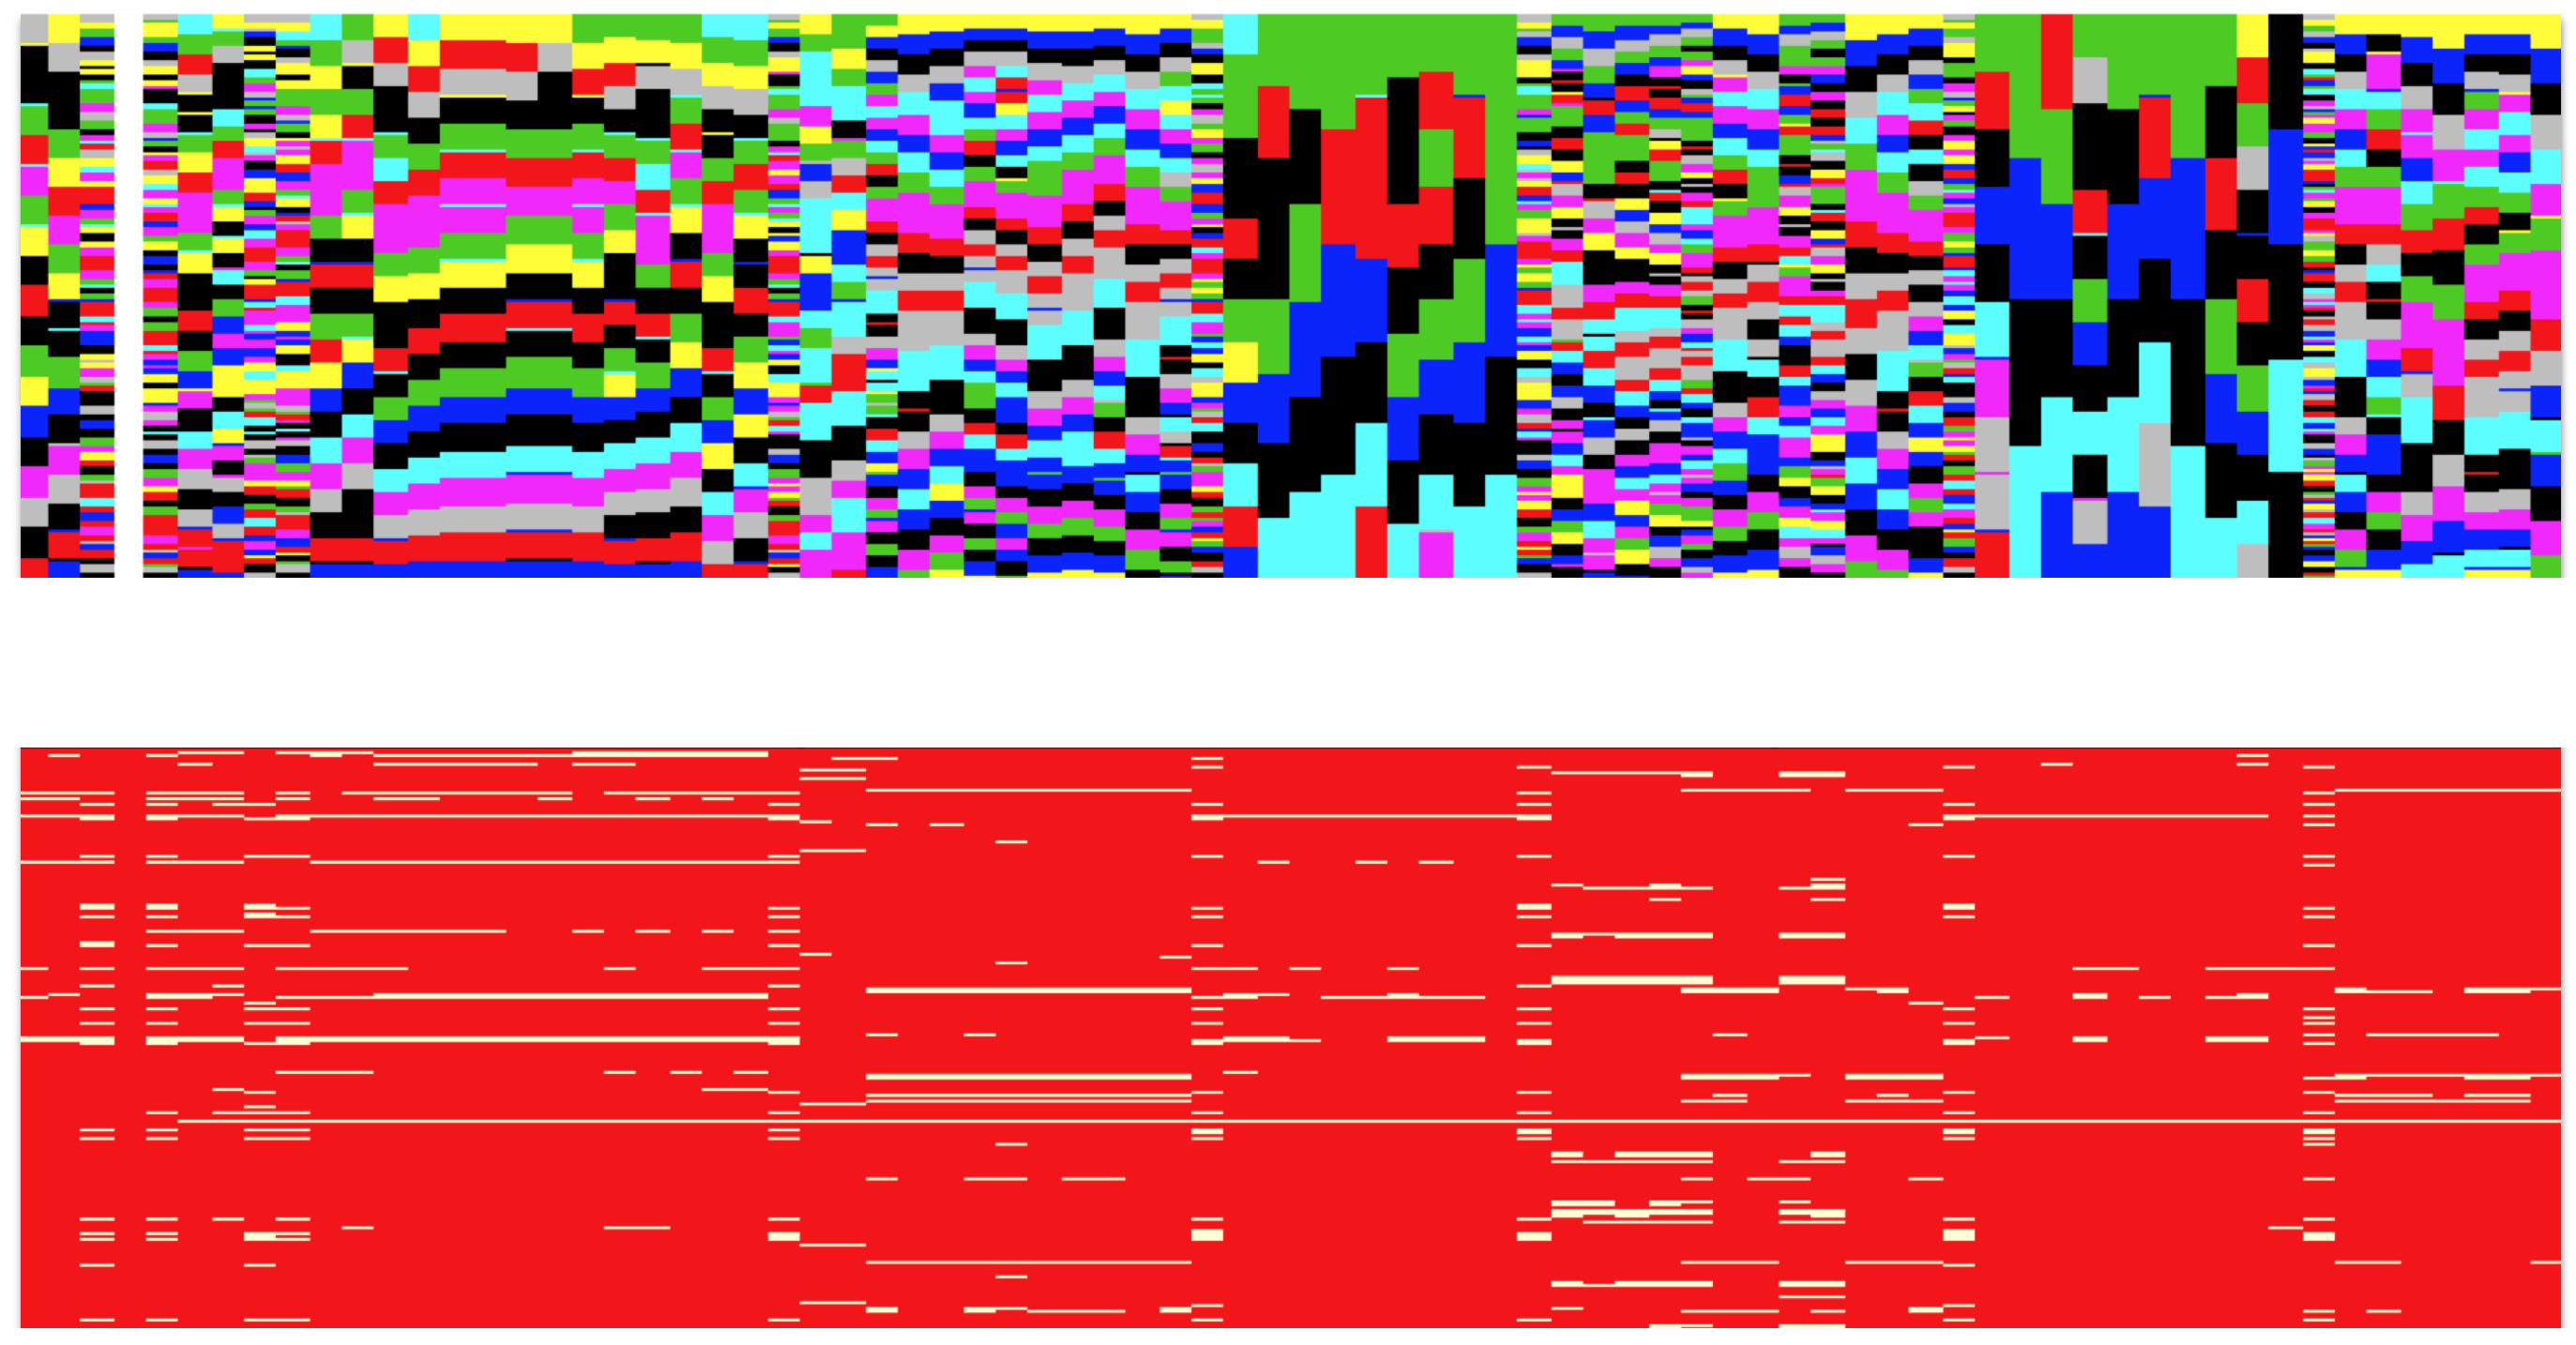
\includegraphics[width=\textwidth]{image.png}
\caption{With a Figure caption}
\label{fig:my_label}
\end{figure}


\section{Exercise 1.3}
And you can even put Python code in here!

\begin{python}
import datetime
print datetime.datetime.now()
\end{python}


\section{Exercise 1.4}
\section{Exercise 1.5}

\section{Exercise 2.1}
\section{Exercise 2.2}
\section{Exercise 2.3}

\section{Exercise 3.1}
\section{Exercise 3.2}
\section{Exercise 3.3}
\section{Exercise 3.4}
\section{Exercise 3.5}

\section{Exercise 4.1}

\end{document}
